\pagebreak
\section{Aufgabe 2: Neuronale Netze}
\subsection{Neuronale Netze mit Numpy}
\subsubsection{Implementierung Backprop mit einem Hidden Layer}
\subsubsection{Hyperparameter}
Im folgenden werden Hyperparameter beschrieben, sowie ihre Auswirkungen auf das Neuronale Netzwerk diskutiert.
\begin{description}
	\item[Anzahl der Neuronen im Hidden Layer]\hfill \\
	\item[Anzahl an Iterationen]\hfill \\
	Die Anzahl der Iterationen, die benötigt werden, bis der Trainingsfehler nicht mehr sinkt, hängt stark von der gewählten Lernrate ab. Im weiteren Verlauf wird das einmalige Iterieren durch den gesamten Trainingsdatensatz als Epoche bezeichnet. In Abbildung \ref*{fig:learning_rates} ist der Trainingsverlauf während mehrerer Epochen für verschiedene Lernraten abgebildet. Bei einer Lernrate von 0.1 sinkt der Trainingsfehler nach 100 Epochen nicht mehr.
	
	\item[Lernrate]\hfill \\
	%TODO: Bezug auf unser Beispiel herstellen
	Die Lernrate $\eta$ reguliert die Auswirkung eines einzelnen Schrittes im Gradientenabstiegsverfahrens. Eine hohes $\eta$ führt zu einer schnellen Minimierung des Trainingsfehlers. Jedoch steig die Gefahr, dass das Verfahren gute Minima überspringt, oder auch um ein gutes Minima Pendelt. Ein kleineres $\eta$ findet mit einer hohen Wahrscheinlichkeit ein besseres Minima, jedoch werden dafür mehr Iterationen benötigt \cite{neuronalenetze}.
	
	In Abbildung \ref*{fig:learning_rates} ist der Trainingsfehler während des Trainingsverlauf bei verschiedenen Lernraten dargestellt. Der Abbildung kann entnommen werden, dass für $\eta=0.01$ das Training nach 300 Epochen immer noch nicht konvergiert ist. Für $\eta=0.2$ ist zu sehen, dass das Verfahren sehr früh konvergiert und daher das Risiko besteht, dass wie oben beschrieben, gute Minima übersprungen wurden. Für komplexere Eingabedaten und Netzwerkarchitekturen würde dies ein reales Problem darstellen. In diesem einfachen Netzwerk und den einfachen Eingabedaten aus der Aufgabenstellung, kann auch mit $\eta=0.2$ ein gutes Ergebnis erreicht werden. Der Mittelweg beider Extreme bildet $\eta=0.1$ und wird als Einstellung vorgenommen.
	
	\begin{figure}[h]
		\centering
		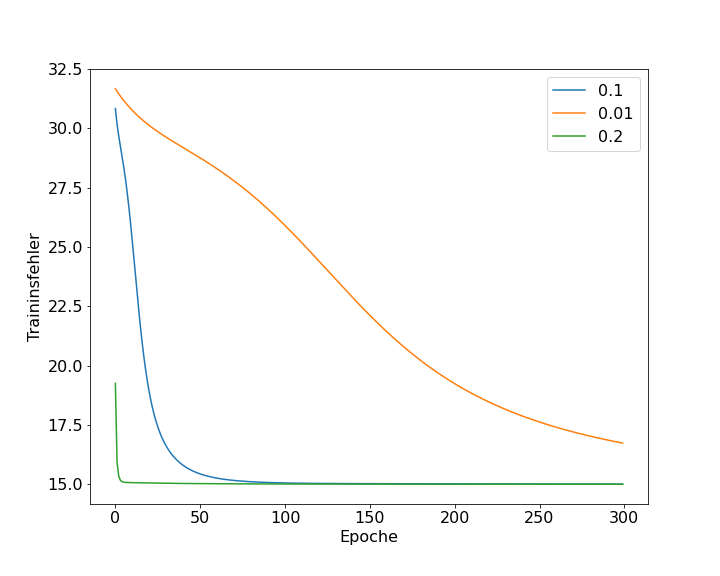
\includegraphics[width = 0.45\textwidth]{Bilder/learning_rates.png}
		\caption{Trainingsfehler während der Trainingsepochen bei verschiedenen Lernraten}
		\label{fig:learning_rates}
	\end{figure}
	
	\item[Initialisierung der Gewichte]\hfill \\
	Vor Allem beim Trainieren von tiefen neuronalen Netzen spielt die Initialisierung der Gewichte eine entscheidende Rolle um das Auftreten des Problems der explodierenden beziehungsweise verschwindenden Gradienten entgegen zu wirken \cite{geron2017hands-on}. In \cite{Glorot10understandingthe} wird die Glorot-Initialisierung, ein Verfahren zur Initialisierung der Gewichte bei Verwendung der Sigmoid Aktivierungsfunktion, beschrieben. Hierbei werden die Werte der initialen Gewichte aus einer Normalverteilung $\mathcal{N}(\mu,\,\sigma^{2})\,$ mit $\mu = 0$ und $\sigma^{2}=\frac{1}{fan_{avg}}$ entnommen. Hierbei gilt: 
	\[
	fan_{avg}=\frac{(fan_{in}+fan_{out})}{2}
	\]
	Wobei $fan_{in}$ der Anzahl an eingehenden Gewichte in einer Schicht entspricht und  $fan_{out}$ der Anzahl an Neuronen in der Schicht. Die Initialisierung der Gewichte in der vorliegenden Arbeit wurde  nach Glorot implementiert.

	%TODO: Muss noch mathematisch und schön. sollten die Schichten und Gewichte mathematisch anotieren. Die anotation dann unter Aufgabe 2.1
	Würden die Gewichte mit Null initialisiert werden, würde der Gradient für Alle Schichten bis auf die Ausgabeschicht Null sein. Ein Lernen würde nicht stattfinden. Der Gradient für die Aktualisierung der Gewichte zwischen versteckter Schicht und Ausgabeschicht würde für alle Partiellen Ableitungen gleich sein. Auch eine Initialisierung mit einer anderen Konstanten würde dazu führen, dass alle Gewichte "auf einer Ebene" gleich aktualisiert werden würden. Sie könnten einfach durch ein Neuron mit einer Verbindung ersetzt werden.
	
	Mithilfe der Verwendung eines \emph{Seeds} wird sicher gestellt, dass die zufällige Initialisierung der Gewichte bei jedem Durchlauf mit den gleichen Parametern die gleichen zufälligen Werte liefert. Das Netzwerk liefert also mit jedem Durchlauf bei gleichen Daten und Parametern die gleichen Ergebnisse. Somit wird die Reproduzierbarkeit im Netzwerk gefördert, was bei einer Fehlersuche und der Hyperparameter Optimierung hilfreich ist.
	
\end{description}
\subsection{Neuronale Netze mit TensorFlow}
%TODO: Tobi
Im Folgenden wird die Implementierung eines voll vernetzen Neuronalen Netzwerks mit Hilfe der \emph{TensorFlow} Bibliothek beschrieben \cite{tensorflow2015-whitepaper}. Unterstützend wurde für den Aufbau des neuronalen Netzes die \emph{Keras}-API verwendet, die seit \emph{TensorFlow} Version 2 standardmäßig integriert ist. 

Um die Daten für das Training des Neuronalen Netzes effizient vorzubereiten wurde die \emph{Dataset}-API verwendet. Mit Hilfe der \emph{Dataset}-API wurde das zufällige Mischen der Trainingsdaten, sowie die Bereitstellung in Form von \emph{Mini-Batches} implementiert. Die Verwendung der \emph{Dataset}-API hat noch zusätzlich den Vorteil, dass die Ausführung von Vorbereitungsschritten der Daten perfekt mit dem Training des Neuronalen Netzes koordiniert und parallelisiert werden können.

\subsubsection{Hyperparameter Suche}
Um ein best Mögliches Modell für die vorliegenden Daten zu finden, wurde eine Hyperparameter-Suche implementiert.
%TODO: Details und halt implementieren.